\acresetall

\chapter{Concept}\label{chapter:concept}
% This chapter introduces the architectural design of Component X. The component consists
% of subcomponent A, B and C.
% In the end of this chapter you should write a specification for your solution, including
% interfaces, protocols and parameters.
This chapter introduces the architectural design of plugin respect to the previously defined requirements.
Therefore the used development environment will be analyzed.
Followed by the initial architecture of the plugin to be developed.
Based on that the different layer of the system will be elaborated.

\section{Overview}
% The concept chapter provides a high-level explanation of your solution. Try to explain
% the overall structure with a picture. You can also use UML sequence diagrams for
% explanation.
% Figure 4.1 illustrates the situation between Alice and Bob. (sequence diagram from
% www.websequencediagrams.com)
\doit

% Docker Plugin as Vim Driver

\section{Development environment}
The choice of the development environment is crucial for the creation of a prototype.
It should be easy to used and fast to implement, but
The environemnt is important for both the implementation of the prototype, as well as the choice of possible plugins and libraries.
Futhermore the prefered environment from the \ac{FOKUS} has to be considered.
Thus, Open Baton is written in Java and is also partly ported to python and go.
Python in general is used for several projects at the \ac{FOKUS}.
Taking also the criterias from section \ref{section:technical-requirements} into account the following programming environments are applicable.
\doit

\textbf{Java:}

\textbf{Python:}

\textbf{Node.js:}

\textbf{Go:}

Due to the fact that python is used for several projects at the \ac{FOKUS} and... % TODO: finish that

The \ac{GUI} is a fundamental web client, which uses Angular.js as its main framework and some smaller tools like jQuery or the pretty famous bootstrap framework.

\section{Architecture of the system}
The overall architecture of the system can be seperated into two levels.
Figure \ref{fig:abstract_architecture_design} will point up the architecture.
The first level is the \textit{centralized fog level}.
This could be for example a cloud server or management node in a fog cluster.
Ideally this level should be implemented with an \ac{MANO} compliant framework.
Hereinafter Open Baton will referred as the tool of choice for that level.
Main function will be the creation of the \ac{NFVI} as well as the deployment of deployment plans for the \acp{NF}.
Open Baton will also have an overview of all existing nodes and can manage and maintain them.

\begin{figure}[H]
    \centering
    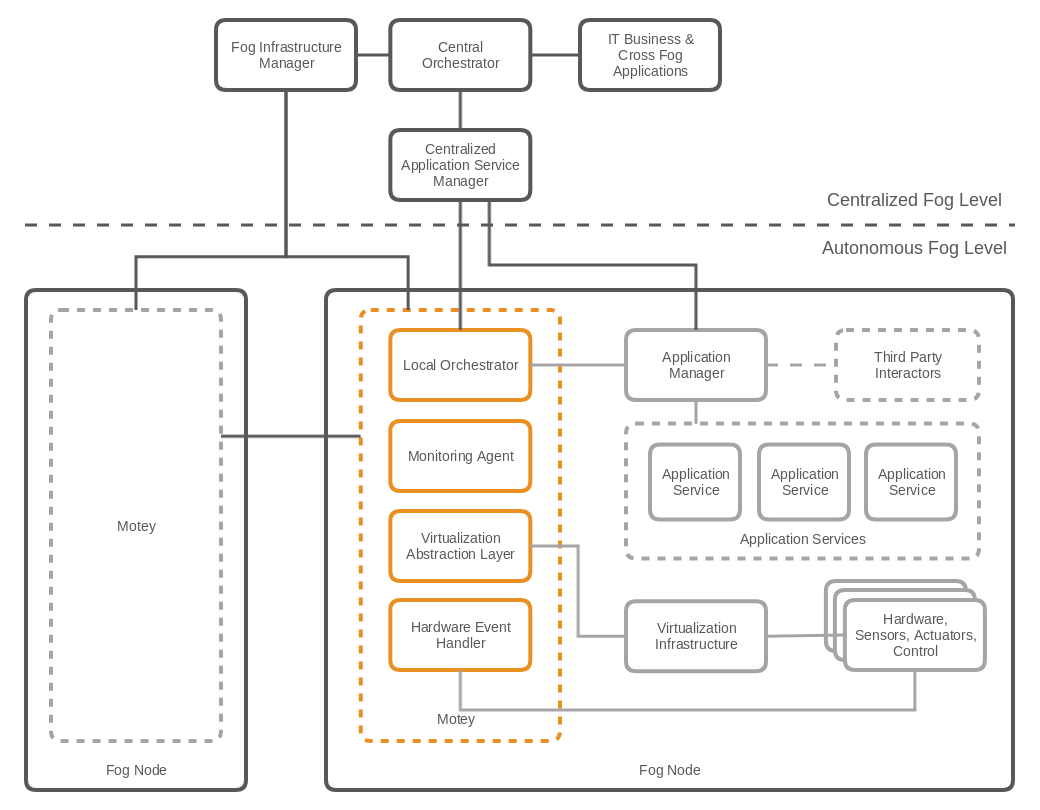
\includegraphics[width=\textwidth]{resources/images/initial_structure.png}
    \caption[Abstract architecture design]{Abstract architecture design}
    \label{fig:abstract_architecture_design}
\end{figure}
% TODO: check if applicaton manager is necessary

The second level is the \textit{autonomous fog level}.
The prototype to be developed will be located in this level.
It includes all existing fog nodes, as well as the prototype referenced as the \textit{OpenIoTFog Agent} in figure \ref{fig:abstract_architecture_design}.
Each node must have a running instance of the OpenIoTFog Agent to be part of the system.
Beside the prototype a node can have several hardware devices, sensors and actuators connected to them.
A virtualization infrastructure such as Docker or XEN, must be installed to be used by the prototype.
These infrastructure can create the containers and \acp{VNF}.
Further it is also possible to have additional third party tools installed which can interact with the them as well.

The OpenIoTFog Agent has several external connection points.
It has a \ac{REST} \ac{API} implemented to get some informations about the status of the fog node, as well as endpoints to receive the deployment plans from centralized fog level.
A \ac{MQTT} connection to a broker, which can be running in the centralized fog level as well as on any other fog node, is used for node discovery.
Finally there are some ZeroMQ endpoints for capability discovery, image deployment and node-to-node communication.
A detailed description will be shown in the following sections.

One of the most important components is the \textit{Local Orchestrator}.
It is responsoible for the deployment of the containers as well as the inter-node communication.
The latter is necessary to let the nodes act in an autonomously was, so that they can react to changing requirements, even when the centralized fog level disappears.
Therefore each node must have knowledge and should be able to interact with each other.
Beside that the local orchestrator is tightly coupled to the \textit{\ac{VAL} Manager}.
This is an abstraction layer for each virtualization component in the system, for example Docker or a bare-metal virtualization like XEN.
These components should be implemented as plugins, so that it is easy to add or remove virtualization components.
Therefore Yapsy\footnote{\url{http://yapsy.sourceforge.net/}} is used as the plugin system of choice.

The \textit{Hardware Event Handler} is a communication endpoint for other third party components.
For example an external hardware listener could send a message to the event handler to register a new connected device like a Zigbee dongle or a bluetooth stick.
This component should allow multiple third party components to send events to them.
Therefore it will be implemented with the publish/subscribe pattern.
Finally the \textit{Monitoring Agenct} is used to log all ongoing events and gives the maintainer of the system an overview of the system processes.
\todo{write more - probabyl about architecture MVC}
% MVC ohne View
% -> keine spezielle architektur
% -> jedoch decoupled as much as possible
% ---> DI, RxPy


\subsection{Data layer}
% daten lesen und schreiben
% tiny db -> easy to use, works well together with json in python
% sollte abstrahiert sein, damit es gut austauschbar ist -> Repository
% config.ini
\doit

\subsection{Orchestration layer}
% ist primär für das Blueprint handling zuständig
% -> bekommt daten via api und parst diese
% -> guckt ob lokal deployed werden kann oder externe Node benötigt wird
% -> yaml als blueprint format
% sowie für die node-to-node Kommunikation
% -> Nodes registrieren sich beim starten der Engine
% -> können capabilities erfragen
% -> können container starten
% -> Sequenzdiagramme für die unterschiedlichen fälle erstellen
\doit

\subsection{Virtualization layer}
The virtualization layer is basically an abstraction layer to generalize the different virtualization engines.
Therefore a so called \ac{VAL} manager which is implemented with the facade design pattern is used to load the plugins and abstract the methods of the plugins.
As mentioned before to realize the plugin functionality the Yapsy library will be used.
The library offers a way to easily add new plugins to the system and is also designed to be easy to use.
It only depends on python standard libraries and lightweight by design.
Each supported virtualization engine needs his own concrete plugin implementation which should be use an interface to have a common ground.
The supported default engine is Docker, but could be extended in a future version of the prototype.

\subsection{Communication layer}
% API für externe tools
% MQTT für node discovery
% ZeroMQ für interne und externe Kommunikation mit einzelnen Komponenten und Tools
% -> beispiel labeling engine und node-to-node Kommunikation
\doit

\subsection{Capability Management}
% labeling engie für hardware events und andere third party apps
% plugins als capability
% werden in db gespeichert
% eine node kann andere nach capabilities fragen -> via ZeroMQ
\doit

\subsection{User interface}
\doit

\subsection{Security}
% Access control
% Encryption of the communcation channels aka REST, ZeroMQ, MQTT
\doit

\section{Conclusion}
\doit




% http://getcloudify.org/brochures/Heavy%20Reading%20NFV%20MANO%20Cloudify%20Snapshot.pdf
